% !TEX encoding = UTF-8
%Koma article
\documentclass[fontsize=12pt,paper=letter,twoside]{scrartcl}
\usepackage{float}
\usepackage{listings}

%Standard Pre-amble
\usepackage[top=4cm,bottom=4cm,left=3cm,right=3cm,asymmetric]{geometry}
%\geometry{landscape}                % Activate for for rotated page geometry
%\usepackage[parfill]{parskip}    % Begin paragraphs with an empty line rather than an indent
\usepackage[table,xcdraw]{xcolor}
\usepackage{graphicx}

\usepackage{amsmath}
\usepackage{amssymb}
\usepackage{epstopdf}
\DeclareGraphicsRule{.tif}{png}{.png}{`convert #1 `dirname #1`/`basename #1 .tif`.png}
% Listings needs package courier
\usepackage{listings} % Needs 
\usepackage{courier}

\usepackage[framemethod=TikZ]{mdframed}
\usepackage{url}

\usepackage{sty/bsymb} %% Event-B symbols
\usepackage{sty/eventB} %% REQ and ENV
\usepackage{sty/calculation}

%Maths
\usepackage{amssymb,amsmath}
\def\Fl{\mathbb{F}}
\def\Rl{\mathbb{R}}
\def\Nl{\mathbb{N}}
\def\Bl{\mathbb{B}}
\def\St{\mathbb{S}}
\newcommand{\ovr}{\upharpoonright}
\newcommand{\var}[1]{\textit{#1}}
%Useful definitions
\newcommand{\mv}[1]{\textit{m\_#1}}
\newcommand{\cv}[1]{\textit{c\_#1}}
\newcommand{\degree}[1]{^{\circ}\mathrm{#1}}
%\newcommand{\comment}[1]{{\footnotesize \quad\texttt{--}\textrm{#1}}}
\newcommand{\im}[1]{i\texttt{-\!#1}}

\usepackage[headsepline]{scrpage2}
\pagestyle{scrheadings}
\ihead[]{\small EECS4312 Report1}
\ohead[]{\small \thepage}
\cfoot[]{}
\ofoot[]{}


%%%%PVS environment%%%%%%%%%%%%%%%%%%%
\lstnewenvironment{pvs}[1][]
    {\lstset{#1,captionpos=b,language=pvs,
    mathescape=true,
    basicstyle=\small\ttfamily,
    numbers=none,
    frame=single,
    % numberstyle=\tiny\color{gray},
    % backgroundcolor=\color{lightgray},
    firstnumber=auto
    }}
    {}
 %%%%%%%%%%%%%%%%%%%%%%%%%%%%%%%%
 
%%%%Verbatim environment%%%%%%%%%%%%%%%%%%%
\lstnewenvironment{code}[1][]
    {\lstset{#1,captionpos=b,
    mathescape=true,
    basicstyle=\small\ttfamily,
    numbers=none,
    frame=single,
    % numberstyle=\tiny\color{gray},
    % backgroundcolor=\color{lightgray},
    firstnumber=auto
    }}
    {}

% \newenvironment{boxed}[1]
%    {\begin{center}
%    #1\\[1ex]
%    \begin{tabular}{|p{0.9\textwidth}|}
%    \hline\\
%    }
%    { 
%    \\\\\hline
%    \end{tabular} 
%    \end{center}
%    }
 %%%%%%%%%%%%%%%%%%%%%%%%%%%%%%%%
 
 %Text in a box
\newenvironment{textbox}
    {\begin{center}
    \begin{tabular}{|p{0.9\textwidth}|}
    \hline\\
    }
    { 
    \\\\\hline
    \end{tabular} 
    \end{center}
    }

\usepackage{hyperref}

%Highlight \hl{}
\usepackage{soul}

\usepackage{enumitem}
\newlist{mylist}{itemize}{1}
\setlist[mylist]{label=\textbullet,leftmargin=1cm,nosep}

\usepackage{multirow}

% Reduce space between figure and caption
%\usepackage{caption}
%\captionsetup[table]{font=small,skip=0pt}     %% Adjust here
%or equivalently 
\usepackage[font=small,skip=4pt]{caption}
%Useful definitions
%\newcommand{\mv}[1]{\textit{m\_#1}}
%\newcommand{\cv}[1]{\textit{c\_#1}}
%\newcommand{\degree}[1]{^{\circ}\mathrm{#1}}
%\newcommand{\comment}[1]{{\footnotesize \quad\texttt{--}\textrm{#1}}}

% Set the header
\ihead[]{\small Gradapps}


%%%%%%%%%%%%Enter your names here%%%%%%%%
\author{\textbf{Edward Vaisman}
\and \textbf{Sadman Sakib Hasan}
}
%%%%%%%%%%%%%%%%%%%%%%%%%%%%%%%%

\date{\today} % Display a given date or no date

\begin{document}
\title{Grad Apps 2.0 \\ System User Manual}
\maketitle

\newpage

%%%%%%%%%%%%%%%%%%%%%%%%%%%%%%%
\tableofcontents

\newpage


%%%%Rest of your document goes here%%%%%%%%%%%%%%%%%%%

\section{General Information}
General Information section explains in general terms the system and the purpose for which it is
intended.

\subsection{System Overview}

GradApps 2.0 is a business system application, which allows, our client to \emph{automate} the selection of the best candidate into the EECS Graduate Program by \emph{minimizing} the manual work to be done. Our client are the members of \textbf{The EECS Graduate Program}.

\bigskip
\noindent The application is broken down into three user levels: \emph{Administrator}, \emph{Committee Member} and \emph{Professor}. Each of the roles play a crucial part in order to select the best candidate into the graduate program. GradApps 2.0 operates as a web application, hence, a reliable internet connection is required when interacting with the application.

\subsection{Organization of the Manual}
The user’s manual consists of eight sections:

\begin{itemize}
\item \textbf{General Information} section explains in general terms the system and the purpose for which it is
intended.
\item \textbf{System Summary} section provides a general overview of the system. The summary outlines the uses of
the system’s hardware and software requirements, system’s configuration, user access levels and
system’s behavior in case of any contingencies.
\item \textbf{Getting Started} section explains how to get GradApps 2.0 and install to have it up and running. This section is solely for administrative uses.
\item \textbf{Using The System} section provides a detailed description of the common system functions.
\item \textbf{Administrator Use} section provides a detailed description of the administrator system functions.
\item \textbf{Committee Member Use} section provides a detailed description of the committee member system functions.
\item \textbf{Professor Use} section provides a detailed description of the professor system functions.
\item \textbf{Help} section provides the contact information for further help on using the application.
\end{itemize}

\newpage
\section{System Summary}
System Summary section provides a general overview of the system. The summary outlines the uses of
the system's hardware and software requirements, system’s configuration, user access levels and
system’s behavior in case of any contingencies.

\subsection{System Configuration} \label{system_conf}

\subsubsection{Browser Configuration}
GradApps 2.0 operates as a web interface application. It supports all modern web browser, however, Chrome and Mozilla Firefox are the recommended browser for using the application. The application is recommended to be only used through desktop browsers.

\bigskip
\noindent\textbf{Recommended Browser(s):}

\begin{itemize}
\item \textbf{Chrome}: $>=$ Chrome v60.0.3112
\item \textbf{Mozilla Firefox}: $>=$ Firefox 57 (v57.0a1)
\end{itemize}

\subsubsection{Node.js Configuration}
GradApps 2.0 is built using Node.js and it is vital to use the correct version of the node package manager (npm) and the node.

\bigskip
\noindent\textbf{Recommended Node.js version:}

\begin{itemize}
\item \textbf{Node}: $>=$ v8.9.4
\item \textbf{NPM}: $>=$ 5.6.0
\end{itemize}

\subsubsection{MySQL Configuration}
GradApps 2.0 uses MySQL commercial database as the datasource manager.

\bigskip
\noindent \textbf{Recommended MySQL version:} $>=$ 5.7.20

\bigskip
\noindent The following environmental variables are required to be set prior to starting the application.

\begin{itemize}
\item \textbf{MYSQL\_HOST}: the host name of the database server
\item \textbf{MYSQL\_PORT}: the port number of the database server
\item \textbf{MYSQL\_USER}: the user name to access the database
\item \textbf{MYSQL\_PASSWORD}: the password to access the database
\item \textbf{MYSQL\_DATABASE}: the database name (optional)
\end{itemize}

\bigskip
\noindent \textbf{Note:} The default database name for the application is \emph{gradapps}. However, any customized database name can be set by using the environmental variable mentioned above.

\subsubsection{Other Configuration}
The default port for the application web server is 3000. However, it can be set to one of your choice by enabling the PORT environmental variable.

\subsection{User Access Levels}
Only registered users can use the application. The user access levels for the three different user roles are discussed further in the document for each role.

\subsection{Contingencies}
In case of power outage or unexpected shutdown of the web server, the application will stop working and any unsaved data will be lost. It is recommended for users to save data frequently to avoid such losses.

\newpage
\section{Getting Started}
Getting Started section explains how to get GradApps 2.0 on the machine, install it and start the application. Please note this section is solely for the system administrator's who will maintain the application.

\bigskip
\noindent To install the application, it has to be pulled from the private GitHub repository as it is not a published application for other uses.

\bigskip
\noindent To clone the repository in the server machine, please make sure Git is installed in the machine. Along with Git, all the above configuration mentioned in Section \ref{system_conf} must be installed.

\bigskip
\noindent \textbf{Recommended Git version:} $>=$ 2.3.2

\smallskip
\begin{enumerate}
\item Git clone the repository in the current working directory, run the following command:
\begin{lstlisting}[language=bash]
  $ git clone https://github.com/ssh24/EECS4090-Project.git
\end{lstlisting}
\item Change the working directory to the source of the project:
\begin{lstlisting}[language=bash]
  $ cd EECS4090-Project/src/
\end{lstlisting}
\item Install the required dependencies:
\begin{lstlisting}[language=bash]
  $ npm install
\end{lstlisting}
\item Set the required environmental variables:
\begin{lstlisting}[language=bash]
  $ SET MYSQL_HOST = <host>
  $ SET MYSQL_PORT = <port>
  $ SET MYSQL_USERNAME = <username>
  $ SET MYSQL_PASSWORD = <password>
  $ SET MYSQL_DATABASE = <database>
  $ SET PORT = <app_port>
\end{lstlisting}
\item Seed the database:
\begin{lstlisting}[language=bash]
  $ npm run seed:app
\end{lstlisting}
\item Start the application server:
\begin{lstlisting}[language=bash]
  $ npm start
\end{lstlisting}
\item The application can then be accessed at port 3000 or the one set by you using the environmental variable. To access the application locally, go to \url{http://localhost:<app_port>}.
\end{enumerate}

\bigskip
\noindent \textbf{Note:} In order for the application be accessible from outside, the application port need to be set open. Once it is set open, the application can be accessed from anywhere it an internet in the following way: \url{http://<app_host>:<app_port>}.

\newpage
\section{Using The System}
section provides a detailed description of the common system functions. Common system functions are functionality that are available to all users who has access to the system. The list of common system functions are listed below:

\subsection{Logging In}

To access the gradapps portal you'll first need to be authenticated into the system. To begin simply click on the ``Sign In" button on the welcome page.

\begin{figure}[!htb]
\begin{center}

\includegraphics[width=.99\textwidth]{images/welcome.png}
\end{center}
\caption{Welcome Page}
\label{fig:welcome}
\end{figure}

\bigskip
\noindent You will then be redirected to the login page. Input your username, password and click on the ``Login" button. If you are successfully authenticated you will be redirected to the role selection page.

\clearpage
\begin{figure}[!htb]
\begin{center}
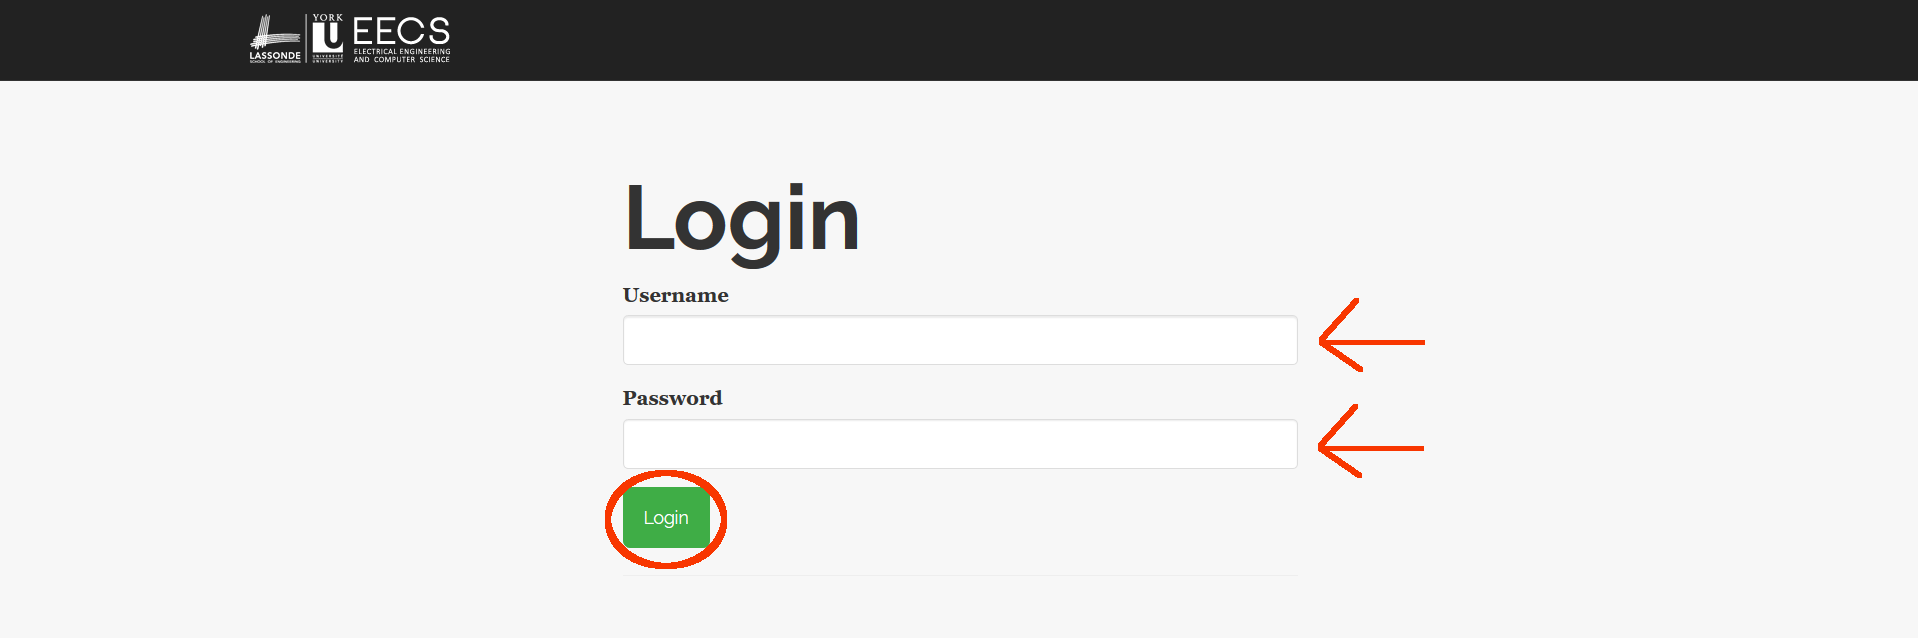
\includegraphics[width=.99\textwidth]{images/login.png}
\end{center}
\caption{Login Page}
\label{fig:login}
\end{figure}

\bigskip
\noindent \textbf{Note:} If the credentials you have provided are invalid you will be greeted with an error message.

\subsection{Selecting a Role}
The subsections below describe the methods for selecting the a role.

\subsubsection{Role Selection Page}
From the role selection page click on the ``Continue as Committee Member" button to be redirected to the committee member portal.

\begin{figure}[!htb]
\begin{center}
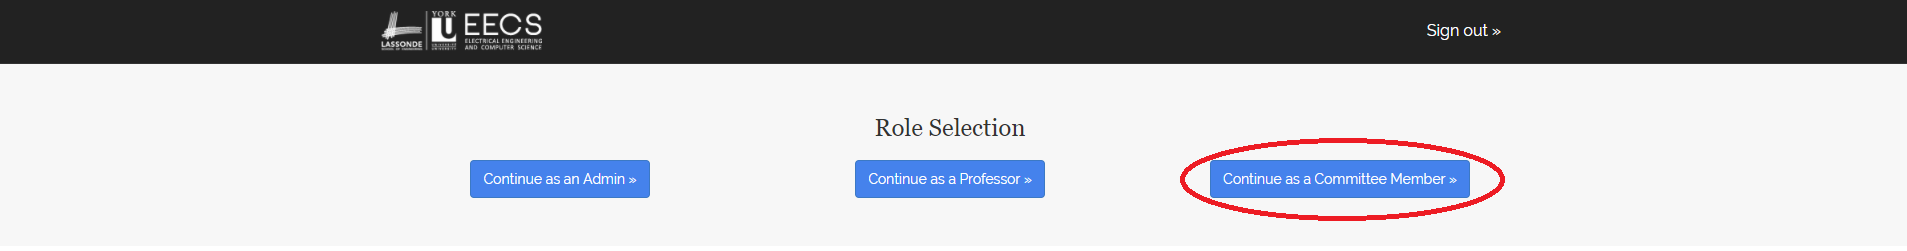
\includegraphics[width=.99\textwidth]{images/auth.png}
\end{center}
\caption{Role Selection Page}
\label{fig:role_selection1}
\end{figure}

\noindent \textbf{Note:} To access the administrator/committee/professor portal you must be granted access from an administrator.

\subsubsection{Navigation Bar}
If you have selected another role and wish to switch roles you will be presented with an option on the navigation bar. Click on the dropdown menu that displays your current role and click on your desired role.
\begin{figure}[!htb]
\begin{center}

\includegraphics[width=.99\textwidth]{images/role-selection2.png}
\end{center}
\caption{Switch Roles}
\label{fig:role_selection2}
\end{figure}

\noindent \textbf{Note:} To access the administrator/committee/professor portal you must be granted access from an administrator.

\subsection{User Settings}
To customize personal user settings, simply click on the ``Settings" button from the navigation bar on any page. The following are the required fields when update personal user settings:
\begin{itemize}
\item Username
\item Last Name
\item First Name
\item Email
\end{itemize}

\begin{figure}[!htb]
\begin{center}
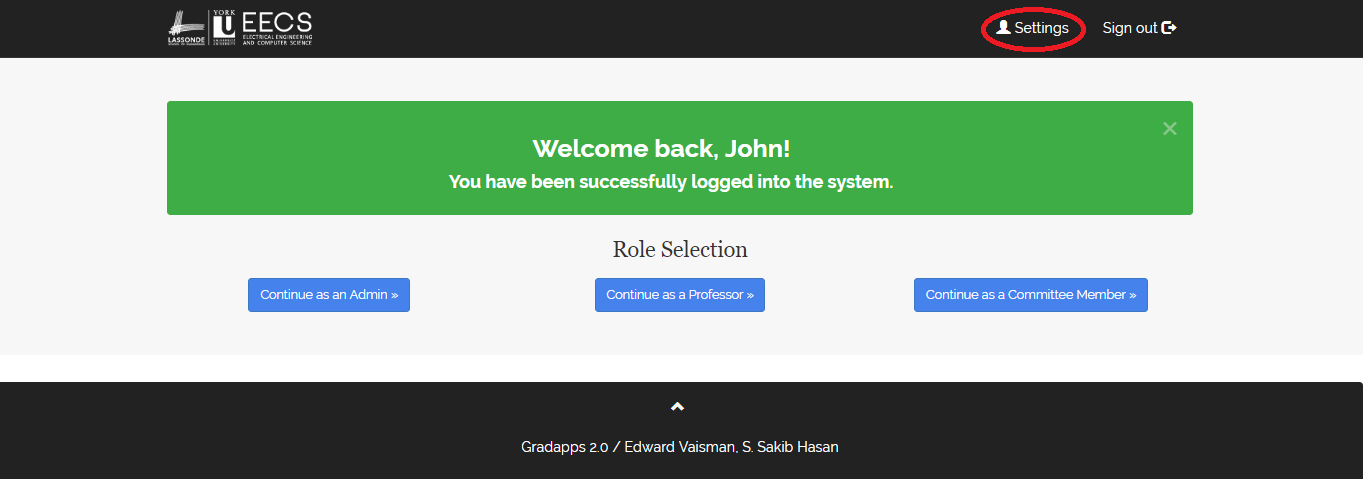
\includegraphics[width=.99\textwidth]{images/click_settings.png}
\end{center}
\caption{Open User Settings}
\label{fig:click_settings}
\end{figure}

\begin{figure}[!htb]
\begin{center}
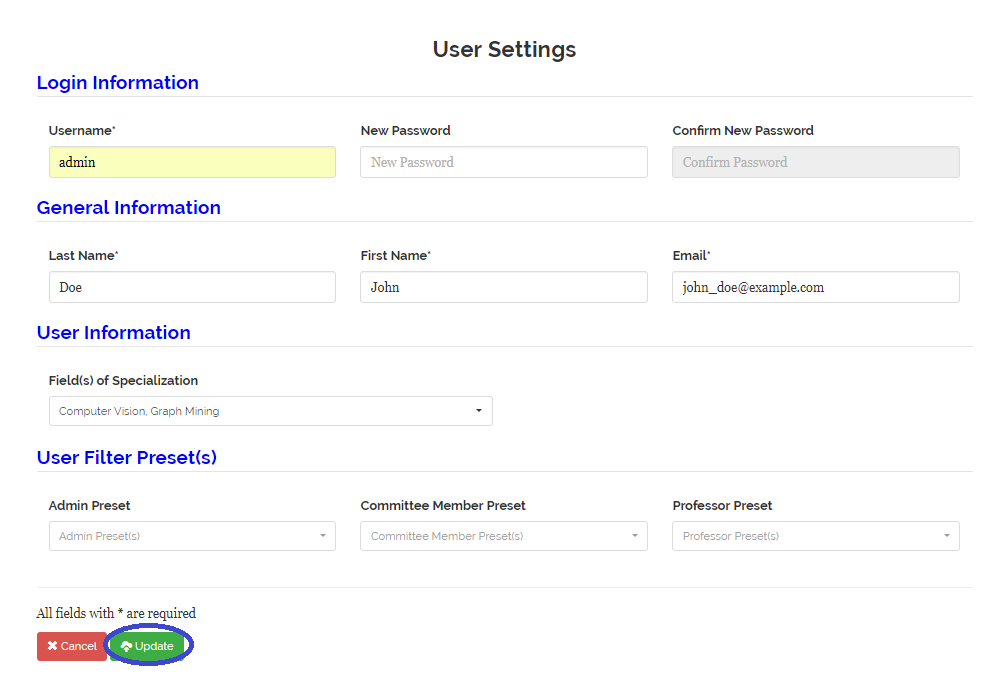
\includegraphics[width=.99\textwidth]{images/settings_form.png}
\end{center}
\caption{User Settings Form}
\label{fig:settings_form}
\end{figure}

\clearpage
\subsection{Logging Out}
To logout of the system, simply click on the ``Sign out" button from the navigation bar on any page.

\bigskip
\noindent \textbf{Note:} Idleness in the system for a maximum of 15 minute will cause the user session to be automatically terminated and the user will be logged out.

\begin{figure}[!htb]
\begin{center}
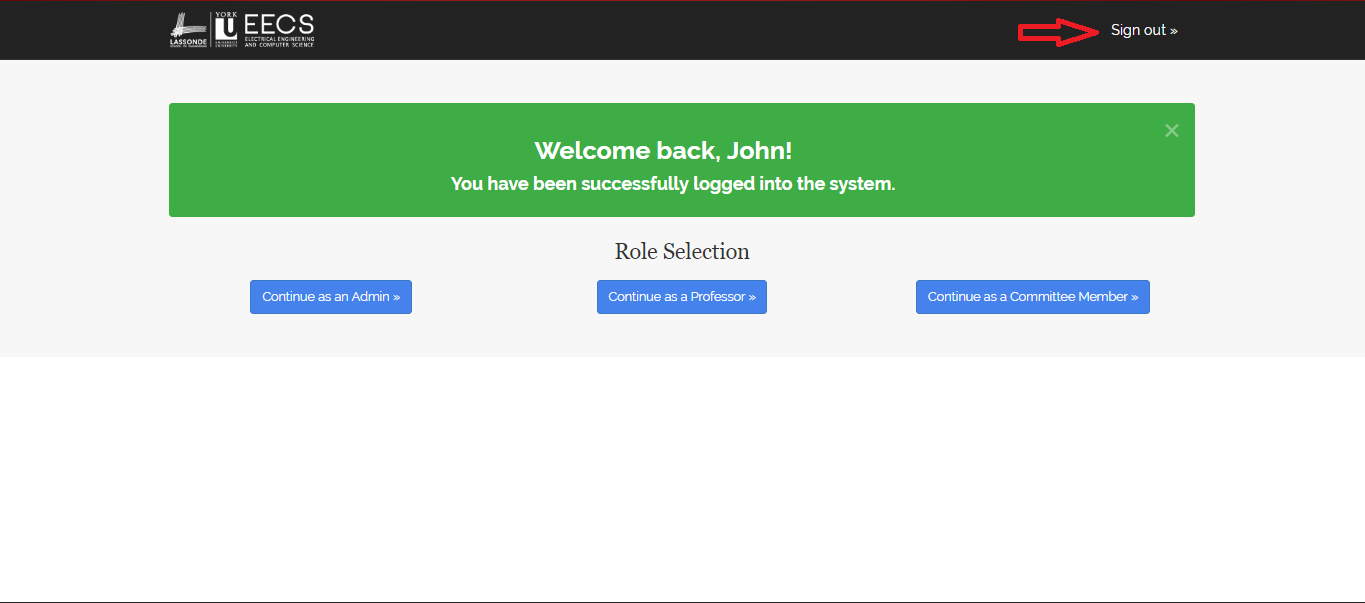
\includegraphics[width=.99\textwidth]{images/logout.png}
\end{center}
\caption{Logout of the System}
\label{fig:logout}
\end{figure}

\newpage
\section{Help}
For further help or information please contact the Graduate Program Director (GPD) or the Graduate Program Assistant (GPA) of the EECS Graduate Program at Lassonde School of Engineering.\\

\begin{center}
\begin{tabular}{ |c |c |c | } \hline
 \textbf{Role} & \textbf{Name} & \textbf{Contact} \\ \hline
 Graduate Program Director & Franck van Breugel & franck@eecs.yorku.ca \\ \hline
 Graduate Program Assistant & Ouma Jaipaul-Gill & gradasst@eecs.yorku.ca \\ \hline
\end{tabular}
\end{center}

\end{document}